%  !TeX  root  =  user_guide.tex

\chapter{Работа с растровыми данными}\label{label_raster}
\index{raster layers|(}

% when the revision of a section has been finalized,
% comment out the following line:
%\updatedisclaimer

Из этой главы вы узнаете, как как вывести растровый слой с различными параметрами.
QGIS поддерживает множество форматов растровых данных. В настоящее время
протестированы следующие форматы:\index{raster layers!data formats}

\begin{itemize}[label=--]
\item Arc/Info Binary Grid
\item Arc/Info ASCII Grid
\item GRASS Raster
\item GeoTIFF
\item JPEG
\item Spatial Data Transfer Standard Grids (с некоторыми ограничениями)
\item USGS ASCII DEM
\item Erdas Imagine
\end{itemize}

Реализация работы с растрами в QGIS основана на библиотеке GDAL, поэтому,
вероятнее всего, другие форматы растров, поддерживаемые GDAL, также будут работать.
В случае сомнения, можно попытаться открыть растр и посмотреть,
поддерживается ли он в QGIS. Больше информации о поддержке растровых
форматов GDAL можно узнать в приложении~\ref{appdx_gdal}
\index{raster layers!GDAL implementation}
или на странице \url{http://www.gdal.org/formats_list.html}. Если вы хотите
загрузить растровые данные в формате GRASS, то обратитесь к
разделу~\ref{sec:load_grassdata}.

\section{Что такое растровые данные?}\label{label_whatsraster}
\index{raster layers!definition}

Растровые данные в ГИС представляют из себя матрицы, каждая ячейка которых
передаёт значение некого параметра поверхности. Каждая ячейка в
растровой сетке имеет определенный размер. Как правило, ячейки имеют
прямоугольную форму (в QGIS они всегда прямоугольные). Типичный набор
растровых данных включает в себя данные дистанционного зондирования,
такие как аэрофотосъемка, спутниковые снимки или смоделированные данные,
например матрицу высот.

В отличии от векторных данных, у растров, как правило, нет присоединенных к каждой
ячейке табличных данных. Они геокодируются размещением пикселей относительно
координат углового пикселя растрового слоя, что позволяет корректно размещать
такие данные на картах в \qg.

Для правильного отображения данных \qg использует информацию о привязке,
находящуюся внутри растрового слоя (например, GeoTiff) или в соответствующем файле
привязки.\index{raster layers!georeferenced}

\section{Загрузка растровых данных в QGIS}\label{label_loadraster}

Растровые слои загружаются нажатием на кнопку
\toolbtntwo{mActionAddRasterLayer}{Загрузить растр} или выбором меню
\mainmenuopt{Слой} >
\dropmenuopttwo{mActionAddRasterLayer}{Добавить растроый слой}.
Несколько слоёв можно загрузить, удерживая клавишу \keystroke{Control}
или \keystroke{Shift} в диалоге \dialog{Добавить растровый слой}.\index{raster layers!loading}

Когда растровый слой появится в панели <<Слои>>, нажмите на нем правой
кнопкой мыши для вызова контекстного меню.

\minisec{Контекстное меню для растровых слоев}

\begin{itemize}[label=--]
\item \dropmenuopt{Увеличить до границ слоя}
\item \dropmenuopt{Увеличить до наилучшего масштаба (100\%)}
\item \dropmenuopt{Показать в обзоре}
\item \dropmenuopt{Удалить}
\item \dropmenuopt{Свойства}
\item \dropmenuopt{Переименовать}
\item \dropmenuopt{Добавить группу}
\item \dropmenuopt{Развернуть все}
\item \dropmenuopt{Свернуть все}
% \item \dropmenuopt{Show file groups} - такого нет.
\end{itemize}

\section{Свойства растра}\label{label_rasterprop}

Чтобы открыть и установить свойства растрового слоя необходимо два раза
кликнуть на нем мышкой в панели <<Слои>> или нажать на растре правой
кнопкой мыши и выбрать \dropmenuopt{Свойства} из контекстного
меню:\index{raster layers!context menu}. На рисунке~\ref{fig:raster_properties}
показано диалоговое окно \dialog{Свойства слоя}. Оно состоит из
вкладок:

\begin{itemize}[label=--]
 \item \tab{Символика}
 \item \tab{Прозрачность}
 \item \tab{Цветовая карта}
 \item \tab{Общие}
 \item \tab{Метаданные}
 \item \tab{Пирамиды}
 \item \tab{Гистограммы}
\end{itemize}

\begin{figure}[h]
  \centering
   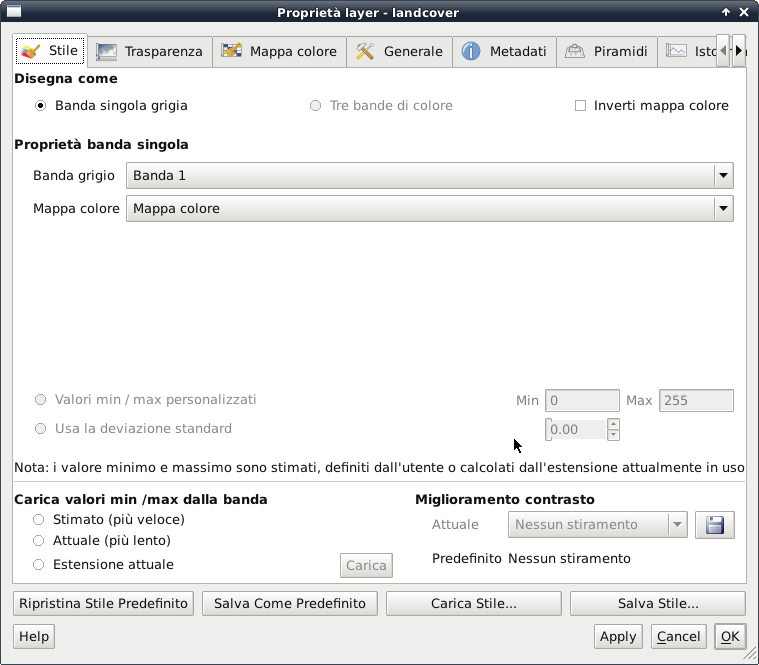
\includegraphics[clip=true, width=14cm]{rasterPropertiesDialog}
   \caption{Свойства растрового слоя \nixcaption}\label{fig:raster_properties}
\end{figure}

\subsection{Символика}\label{label_symbology}

В QGIS есть два способа отображения растрового слоя:\index{raster layers!supported channels}

\begin{itemize}[label=--]
\item Одноканальное серое --- изображение будет выведено в оттенках серого
или в псевдоцветном режиме. % еще в кислотном и цветовой картой
\item Трехканальное цветное --- растр отображается в виде трех каналов:
красный, зелёный и синий, которые используются для создания цветного
изображения.
\end{itemize}

В обоих типах отображения можно инвертировать цвета, используя флажок
\checkbox{Обратить цветовую карту}. %может лучше "гамму"?

\minisec{Одноканальное отображение}

Этот режим включает два основных параметра. Во-первых, вы можете выбрать канал,
который нужно отобразить (если данные состоят из нескольких каналов).

Во-вторых, вы можете выбрать для отображения одну из имеющихся цветовых схем.

В выпадающем списке выбора цветовой карты доступны следующие пункты:
\selectstring{{}Цветовая карта}{Градации серого} --- по умолчанию выбраны градации серого. Также доступны режимы:
\begin{itemize}[label=--]
\item Псевдоцвет
\item Кислотная
\item Цветовая карта
\end{itemize}

При выборе режима \selectstring{{}Цветовая карта}{Цветовая карта}, становится
доступной вкладка \tab{Цветовая карта}. Цветовая карта подробно рассматривается в разделе~\ref{label_colormaptab}.

QGIS может скрывать пиксели, значения которых находятся вне заданного
интервала стандартного отклонения от среднего по слою.\index{raster layers!standard deviation}
Эта функция применяется, когда в растровом слое присутствуют несколько ячеек
с ошибочно завышенными значениями, которые негатино влияют на отображение растра.
Данный параметр доступен только для выводимых в псевдоцвете изображений.

\minisec{Трёхканальное отображение}

Этот режим позволяет более гибко изменять внешний вид растрового слоя.
Например, можно изменить порядок цветовых каналов со стандартной RGB-схемы на
какой-нибудь другой.

Для цветовых каналов допускается масштабирование значений.


\begin{Tip}\caption{\textsc{Просмотр одного канала многоканального растра}}
Для того, чтобы отобразить только один канал (например, красный) в
многокальном изображении, можно задать каналы зелёного и синего в значение
<<Не задано>>, но это не совсем корректно. Для отображения красного
канала нужно задать тип отображения в <<Градации серого>>, а затем
выбрать красный как основной канал для серого.
\end{Tip}

\subsection{Прозрачность} \label{rastertab:transparency}

QGIS поддерживает отображение растровых слоёв с разной степенью
прозрачности.\index{raster layers!transparency} Для этого используется
ползунок прозрачности, с помощью которого можно указать, до какой
степени слой может быть прозрачным, чтобы увидеть слои, находящиеся под
ним. Это очень удобно, когда загружено множество растровых слоев,
например растр с изображением рельефа и основной растр. Это позволит
сделать внешний вид карты более трехмерным.

Также, можно ввести величину растра, которая будет рассматриваться
как значение {\em <<НЕТ ДАННЫХ>>}.

Более гибко степень прозрачности можно настроить в панели
\guiheading{Параметры прозрачности}, которая позволяет указать индивидуальную
прозрачность каждого пикселя.

Например, нужно установить прозрачность воды в растре
\filename{landcover.tif} 20\%. Для этого нужно:
\begin{enumerate}
 \item Загрузить растр \filename{landcover}
 \item Открыть \dialog{Свойства} растра двойным щелчком на имени растра в легенде
 или щёлкнув на нём правой кнопкой мыши и выбрать \dropmenuopt{Свойства}
 из контекстного меню.
 \item Выбрать вкладку \tab{Прозрачность}
 \item \label{enum:add} Нажать кнопку
 \toolbtntwo{mActionNewAttribute}{Добавить значения вручную}. Появится
 новая строка в перечне прозрачных пикселей
 \item \label{enum:transp} Ввести значение растра (например, 0) и
 установить значение прозрачности в 20\%
 \item Нажать \button{Применить} и посмотреть результат на карте
\end{enumerate}

Можно повторить шаги \ref{enum:add} и \ref{enum:transp} чтобы добавить
больше значений для задания прозрачности.

Как видно, настройка прозрачности растра "--- простая, но требующая времени
процедура. Для экономии времени в дальнейшем можно воспользоваться кнопкой
\toolbtntwo{mActionFileSave}{Экспорт в файл} для сохранения заданных
параметров. Кнопка \toolbtntwo{mActionAddRasterLayer}{Импорт из файла}
загружает сохранённые ранее параметры прозрачности и применяет их к
выбранному растровому слою.

\subsection{Цветовая карта} \label{label_colormaptab}
% FIXME: Write me

Вкладка \tab{Цветовая карта} доступна при выборе одноканального режима
отображения растра во вкладке \tab{Символика} (см. главу~\ref{label_symbology}).

Доступны три вида интерполяции цветов:
\begin{itemize}[label=--]
\item Дискретная
\item Линейная
\item Точечная
\end{itemize}

Кнопка \button{Добавить значение} добавляет цвет в пользовательскую таблицу
цветов. Двойной щелчок мыши на поле <<Значение>>
позволяет задать конкрентую величину, соответствующую данному цвету. Двойной щелчок
мыши на поле <<Цвет>> открывает диалоговое окно \dialog{Выбор цвета}, в котором
можно выбрать цвет для данной величины.

Кнопка \toolbtntwo{mActionNewAttribute}{Загрузить цветовую карту из канала},
позволяет загрузить таблицу цветов из канала (если она в нём присутствует).

Блок \guiheading{Создать новую цветовую карту} позволяет создавать
новые категории цветовой карты. Для этого задается нужное
\selectnumber{{}количество значений}{15} и нажимается кнопка
\button{Классифицировать}. В настоящее время поддерживается только
\selectstring{{}Режим классификации}{Равные интервалы}\index{raster layer!classify}.

\subsection{Общие}\label{label_generaltab}

Вкладка \tab{Общие} содержит основную информацию о выбранном растре,
в том числе источник слоя и его имя в легенде (которое можно изменить).
Также, в этой вкладке отображается образец слоя, его легенда и палитра.
\index{raster layers!properties}

Кроме того, в этой вкладке можно установить видимость слоя в пределах
масштаба. Для этого нужно установить флажок в соответствующем поле и
задать масштаб, в пределах которого данный слой будет видим на
карте.

Также здесь показана система коородинат в виде строки PROJ.4. Для её изменения
нажмите кнопку \button{Выбрать}.

\subsection{Метаданные}\label{label_metatab}

Вкладка \tab{Метаданные} содержит полные данные о растровом слое,
включая статистику о каждом канале загруженного растра. Статистические
данные собираются по принципу <<нужно знать>>, так что, возможно,
статистика по слоям может быть не доступной.\index{raster layers!metadata}

В основном, эта вкладка используется для просмотра информации. В ней
нельзя изменить какие-либо значения. Для обновления статистики нужно
перейти на вкладку \tab{Гистограмма} и нажать кнопку \button{Обновить}.
Подробнее о гистограммах говорится в разделе~\ref{label_histogram}.

\subsection{Пирамиды}\label{raster_pyramids}

Растры высокого разрешения могут замедлить навигацию в QGIS. Создание
копий данных низкого разрешения (пирамид) позволяет существенно повысить
скорость, поскольку QGIS будет автоматически выбирать оптимальное
разрешение в зависимости от текущего масштаба.
\index{raster layers!pyramids}
\index{raster layers!resolution pyramids}

Для сохранения пирамид необходимы права на запись в каталог, в котором
хранятся оригинальные данные. \\
Для построения пирамид используются два метода интерполяции:
\begin{itemize}[label=--]
\item Среднее значение
\item Ближайший сосед
\end{itemize}

Если активен флажок
\checkbox{Создавать встроенные пирамиды, если возможно} QGIS будет
пытаться создать внутренние пирамиды.

Обратите внимание, что операция построения встроенных пирамид может
изменить оригинальный файл данных и их невозможно будет удалить после
создания. Поэтому перед построением пирамид рекомендуется сделать резервную копию
растровых данных.

\subsection{Гистограмма}\label{label_histogram}

Вкладка \tab{Гистограмма} позволяет просмотреть распределение \index{raster layers!histogram}
каналов или цветов в растре. Для начала нужно создать статистику растра,
нажав на кнопку \button{Обновить}. Отдельные каналы для
отображения можно выбрать из списка. Доступно два вида диаграмм:

\begin{itemize}[label=--]
\item Столбчатая
\item Линейная
\end{itemize}

Также, можно задать количество столбцов диаграммы и режим отображения:
\checkbox{Разрешить аппроксимацию} или \checkbox{Разрешить значения вне диапозона}.
После просмотра гистограммы можно заметить, что поля статистики каналов
на вкладке \tab{Метаданные} будут заполнены.\index{raster layers!metadata)}

\begin{Tip}\caption{\textsc{Сбор статистики растра}}
Для сбора статистики по слою, выберите псевдоцветное преобразование и
нажмите \button{Применить}. Сбор статистики может занять продолжительное
время. Дождитесь, пока QGIS обработает ваши данные!\index{raster layers!statistics}
\end{Tip}

\FloatBarrier
